\documentclass[UTF8]{ctexrep}
\usepackage[CJKbookmarks,pdfpagemode=UseOutlines,bookmarksnumbered,bookmarksopen]{hyperref}
\hypersetup{
    colorlinks=true,
    linkcolor=black
}
\usepackage{amsmath}
\usepackage{geometry}
\usepackage{booktabs}
\usepackage{longtable}
\usepackage{pdflscape}
\usepackage{multirow}
\geometry{a4paper,centering,scale=0.8}
\usepackage{xcolor}
\usepackage{fontspec}
\newfontfamily\cour{cour.ttf}
\usepackage{listings}
\lstset{
    numbers=left,
    basicstyle= \small\cour,
    numberstyle= \tiny\cour,
    keywordstyle= \color{ blue!70},
    commentstyle= \color{green!100},
    frame=shadowbox, % 阴影效果
    rulesepcolor= \color{ red!20!green!20!blue!20} ,
    escapeinside=``, % 英文分号中可写入中文
    xleftmargin=2em,xrightmargin=2em, aboveskip=1em,
    framexleftmargin=2em
}
\CTEXsetup[name={\S,},number={\arabic{chapter}}]{chapter}
\usepackage{graphicx}
\usepackage{float}
\usepackage{subfigure}
\usepackage{enumitem}
\usepackage{ragged2e}
\usepackage{fancyhdr}
\makeatletter
\newcommand\dlmu[2][4cm]{\hskip1pt\underline{\hb@xt@ #1{\hss#2\hss}}\hskip3pt}
\makeatother

\title{计算机组成原理—CPU}
\author{2017303134\ -\ 14011706\ -\ 李太吉}

\newlength{\drop}

\begin{document}

\begin{titlepage}
\drop=0.1\textheight
\centering
\settowidth{\unitlength}{\LARGE 计算机组成原理—Intel芯片介绍}
\vspace*{\baselineskip}
\rule{\unitlength}{1.6pt}\vspace*{-\baselineskip}\vspace*{2pt}
\rule{\unitlength}{0.4pt}\\[\baselineskip]
{\LARGE CPU设计报告}\\[\baselineskip]
{\itshape 计算机组成原理大作业}\\[0.2\baselineskip]
\rule{\unitlength}{0.4pt}\vspace*{-\baselineskip}\vspace{3.2pt}
\rule{\unitlength}{1.6pt}\\[\baselineskip]
\vspace{0.2\textheight}
\Large{姓名:\dlmu{\textsc{李太吉}}\\
班级:\dlmu{\textsc{14011706}}\\
学号:\dlmu{\textsc{2017303134}}\\
学院:\dlmu{\textsc{软件学院}}}\\[\baselineskip]
\vfill

\includegraphics[scale=0.15]{timg.jpg}\par
{\large\scshape 西北工业大学软件学院}\\[\baselineskip]
{\small\scshape 2019年6月4日}\par
\vspace*{\drop}
\end{titlepage}
\tableofcontents

\chapter{指令分析}

\section{指令集}

我们要实现的CPU所应支持的指令集为以下8条指令。
\begin{lstlisting}[language={[x86masm]Assembler}]
mov dest,sour;[sour]- > [dest]
add dest,sour;[dest]+ = [sour]
sub dest,sour;[dest]- = [sour]
and dest,sour;[dest]& = [sour]
or dest,sour;[dest]|= [sour]
not dest;[dest] = [dest]
jmp tar;Jump to tar to run
hlt; halt but not shutdown computer
\end{lstlisting}

\section{指令集要求}
指令集的要求和CPU的寻址特点为:
\begin{enumerate}
\item 支持0 操作数、单操作数和双操作数三种指令
\item 所有指令的两个操作数不能同时为内存操作数
\item 支持立即寻址、直接寻址、寄存器直接寻址和相对寻址四种寻址方式
\item 采用1字节或者2字节变长指令字,操作码采用定长格式
\item CPU字长为8位,8个程序员可见的寄存器,分别命名为$\mathrm{r_0,\cdots,r_7}$
\item 地址总线、数据总线各为8位,可访问$2^8$字节的地址空间
\end{enumerate}

\section{指令格式分析}

首先,我们分析这8条指令。我们用reg代表寄存器,mem代表存储器,A代表立即数。考察8条指令的具体格式。

\subsection{mov指令}

\begin{lstlisting}[language={[x86masm]Assembler}]
mov reg,reg;`寄存器->寄存器,寄存器直接寻址`
mov reg,mem;`存储器->寄存器,寄存器直接寻址和直接寻址`
mov mem,reg;`寄存器->存储器,寄存器直接寻址和直接寻址`
\end{lstlisting}

\subsection{add指令}

\begin{lstlisting}[language={[x86masm]Assembler}]
add reg,reg;`寄存器->寄存器,寄存器直接寻址`
add reg,mem;`存储器->寄存器,寄存器直接寻址和直接寻址`
\end{lstlisting}

\subsection{sub指令}

\begin{lstlisting}[language={[x86masm]Assembler}]
sub reg,reg;`寄存器->寄存器,寄存器直接寻址`
sub reg,mem;`存储器->寄存器,寄存器直接寻址和直接寻址`
\end{lstlisting}

\subsection{and指令}

\begin{lstlisting}[language={[x86masm]Assembler}]
and reg,reg;`寄存器->寄存器,寄存器直接寻址`
and reg,mem;`存储器->寄存器,寄存器直接寻址和直接寻址`
\end{lstlisting}

\subsection{or指令}

\begin{lstlisting}[language={[x86masm]Assembler}]
or reg,reg;`寄存器->寄存器,寄存器直接寻址`
or reg,mem;`存储器->寄存器,寄存器直接寻址和直接寻址`
\end{lstlisting}

\subsection{not指令}

\begin{lstlisting}[language={[x86masm]Assembler}]
not reg;`寄存器,寄存器直接寻址`
\end{lstlisting}

\subsection{jmp指令}

\begin{lstlisting}[language={[x86masm]Assembler}]
jmp A;`立即数,相对寻址`
\end{lstlisting}

\chapter{指令格式设计}

指令集共有8条指令,操作码定长,所以我们规定操作码(OP)占3位,寻址模式有4种,则用2位寻址特征来代表,CPU地址空间为$2^8$字节,则每个地址码占8位,寄存器共有8个,故寄存器编号为3位。

我们规定操作码和寻址特征如下:

\section{操作码}

\begin{table}[H]
\centering
\begin{tabular}{|c|c|}
\hline
指令  & 操作码 \\ \hline
mov & 000 \\ \hline
add & 001 \\ \hline
sub & 010 \\ \hline
add & 011 \\ \hline
or  & 100 \\ \hline
not & 101 \\ \hline
jmp & 110 \\ \hline
hlt & 111 \\ \hline
\end{tabular}
\caption{各指令的操作码}
\label{tab:1}
\end{table}

\section{寻址特征}

\begin{table}[H]
\centering
\begin{tabular}{|c|c|}
\hline
寻址方式    & 寻址特征 \\ \hline
reg-reg & 00   \\ \hline
reg-mem & 01   \\ \hline
mem-reg & 10   \\ \hline
reg     & 11   \\ \hline
\end{tabular}
\caption{寻址特征}
\label{tab:2}
\end{table}

综合以上分析,我们设计这八条指令具体格式如下。

\section{指令格式}

\subsection{mov指令}

mov指令一共有四种。
\begin{enumerate}
\item reg-reg
\begin{table}[H]
\centering
\begin{tabular}{|c|c|c|c|c|}
\hline
OP        & M        & R1   & R2   & ADD  \\ \hline
000(3bit) & 00(2bit) & 3bit & 3bit & 5bit \\ \hline
\end{tabular}
\caption{mov: reg-reg}
\label{tab:3}
\end{table}

\item reg-mem
\begin{table}[H]
\centering
\begin{tabular}{|c|c|c|c|c|}
\hline
OP        & M        & R    & MEM  \\ \hline
000(3bit) & 01(2bit) & 3bit & 8bit \\ \hline
\end{tabular}
\caption{mov: reg-mem}
\label{tab:4}
\end{table}

\item mem-reg
\begin{table}[H]
\centering
\begin{tabular}{|c|c|c|c|c|}
\hline
OP        & M        & R   & MEM  \\ \hline
000(3bit) & 10(2bit) & 3bit & 8bit \\ \hline
\end{tabular}
\caption{mov: mem-reg}
\label{tab:5}
\end{table}
\item reg-立即数
\begin{table}[H]
\centering
\begin{tabular}{|c|c|c|c|c|}
\hline
OP        & M        & R    & 立即数  \\ \hline
000(3bit) & 11(2bit) & 3bit & 8bit \\ \hline
\end{tabular}
\caption{mov: reg-立即数}
\label{tab:6}
\end{table}

\end{enumerate}
\textbf{注:}ADD字段为指令字长的补齐字段,无意义。

\subsection{add指令}
add指令有三种。

\begin{enumerate}
\item reg-reg
\begin{table}[H]
\centering
\begin{tabular}{|c|c|c|c|c|}
\hline
OP        & M        & R1   & R2   & ADD  \\ \hline
001(3bit) & 00(2bit) & 3bit & 3bit & 5bit \\ \hline
\end{tabular}
\caption{add: reg-reg}
\label{tab:7}
\end{table}

\item reg-mem
\begin{table}[H]
\centering
\begin{tabular}{|c|c|c|c|c|}
\hline
OP        & M        & R    & MEM  \\ \hline
001(3bit) & 01(2bit) & 3bit & 8bit \\ \hline
\end{tabular}
\caption{add: reg-mem}
\label{tab:8}
\end{table}

\item reg-立即数
\begin{table}[H]
\centering
\begin{tabular}{|c|c|c|c|c|}
\hline
OP        & M        & R    & 立即数  \\ \hline
001(3bit) & 10(2bit) & 3bit & 8bit \\ \hline
\end{tabular}
\caption{add: reg-立即数}
\label{tab:9}
\end{table}

\end{enumerate}

\subsection{sub指令}
sub指令有三种。

\begin{enumerate}
\item reg-reg
\begin{table}[H]
\centering
\begin{tabular}{|c|c|c|c|c|}
\hline
OP        & M        & R1   & R2   & ADD  \\ \hline
010(3bit) & 00(2bit) & 3bit & 3bit & 5bit \\ \hline
\end{tabular}
\caption{sub: reg-reg}
\label{tab:10}
\end{table}

\item reg-mem
\begin{table}[H]
\centering
\begin{tabular}{|c|c|c|c|c|}
\hline
OP        & M        & R    & MEM  \\ \hline
010(3bit) & 01(2bit) & 3bit & 8bit \\ \hline
\end{tabular}
\caption{sub: reg-mem}
\label{tab:11}
\end{table}

\item reg-立即数
\begin{table}[H]
\centering
\begin{tabular}{|c|c|c|c|c|}
\hline
OP        & M        & R    & 立即数  \\ \hline
010(3bit) & 10(2bit) & 3bit & 8bit \\ \hline
\end{tabular}
\caption{sub: reg-立即数}
\label{tab:12}
\end{table}

\end{enumerate}

\subsection{and指令}
and指令有三种。

\begin{enumerate}
\item reg-reg
\begin{table}[H]
\centering
\begin{tabular}{|c|c|c|c|c|}
\hline
OP        & M        & R1   & R2   & ADD  \\ \hline
100(3bit) & 00(2bit) & 3bit & 3bit & 5bit \\ \hline
\end{tabular}
\caption{and: reg-reg}
\label{tab:13}
\end{table}

\item reg-mem
\begin{table}[H]
\centering
\begin{tabular}{|c|c|c|c|c|}
\hline
OP        & M        & R    & MEM  \\ \hline
100(3bit) & 01(2bit) & 3bit & 8bit \\ \hline
\end{tabular}
\caption{and: reg-mem}
\label{tab:14}
\end{table}

\item reg-立即数
\begin{table}[H]
\centering
\begin{tabular}{|c|c|c|c|c|}
\hline
OP        & M        & R    & 立即数  \\ \hline
100(3bit) & 10(2bit) & 3bit & 8bit \\ \hline
\end{tabular}
\caption{and: reg-立即数}
\label{tab:15}
\end{table}

\end{enumerate}

\subsection{or指令}
or指令有三种。

\begin{enumerate}
\item reg-reg
\begin{table}[H]
\centering
\begin{tabular}{|c|c|c|c|c|}
\hline
OP        & M        & R1   & R2   & ADD  \\ \hline
101(3bit) & 00(2bit) & 3bit & 3bit & 5bit \\ \hline
\end{tabular}
\caption{or: reg-reg}
\label{tab:16}
\end{table}

\item reg-mem
\begin{table}[H]
\centering
\begin{tabular}{|c|c|c|c|c|}
\hline
OP        & M        & R    & MEM  \\ \hline
101(3bit) & 01(2bit) & 3bit & 8bit \\ \hline
\end{tabular}
\caption{and: reg-mem}
\label{tab:17}
\end{table}

\item reg-立即数
\begin{table}[H]
\centering
\begin{tabular}{|c|c|c|c|c|}
\hline
OP        & M        & R    & 立即数  \\ \hline
101(3bit) & 10(2bit) & 3bit & 8bit \\ \hline
\end{tabular}
\caption{or: reg-立即数}
\label{tab:18}
\end{table}

\end{enumerate}

\subsection{not指令}
not指令有一种。
\begin{table}[H]
\centering
\begin{tabular}{|c|c|c|}
\hline
OP        & M        & R    \\ \hline
101(3bit) & 00(2bit) & 3bit \\ \hline
\end{tabular}
\caption{not: reg}
\label{tab:19}
\end{table}

\subsection{jmp指令}
jmp指令有一种。
\begin{table}[H]
\centering
\begin{tabular}{|c|c|c|}
\hline
OP        & A(立即数) \\ \hline
110(3bit) & 5bit   \\ \hline
\end{tabular}
\caption{jmp: A}
\label{tab:20}
\end{table}

\subsection{hlt指令}
hlt指令有一种。
\begin{table}[H]
\centering
\begin{tabular}{|c|c|c|}
\hline
OP        & ADD \\ \hline
110(3bit) & 5bit   \\ \hline
\end{tabular}
\caption{hlt}
\label{tab:21}
\end{table}

\chapter{CPU逻辑框图}

\begin{figure}[H]
\centering
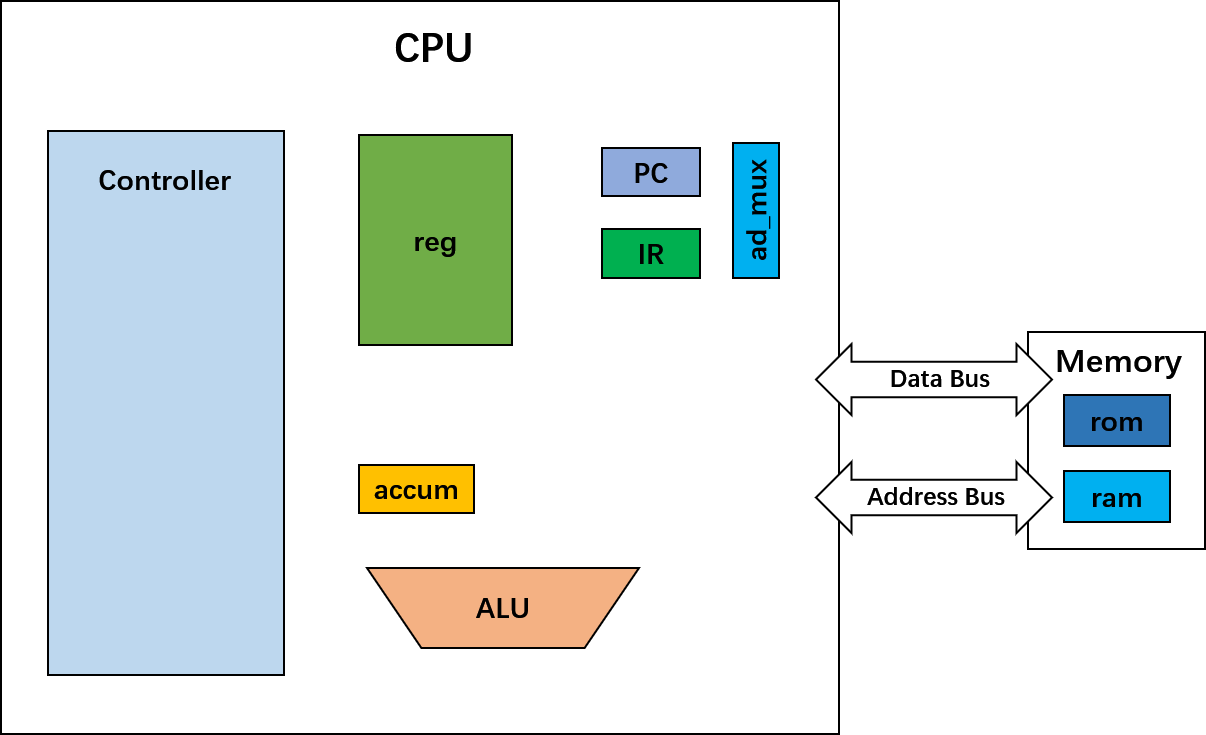
\includegraphics[scale=0.6]{CPU-comp-right.png}
\caption{组合逻辑CPU框图}
\end{figure}

\begin{figure}[H]
\centering
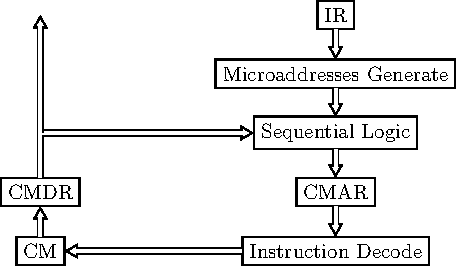
\includegraphics[scale=1.5]{pic.pdf}
\caption{微程序设计CPU框图}
\end{figure}

\chapter{组合逻辑设计}

\section{操作时间表}
由于部分指令字长为16位,而机器字长和存储字长为8位,所以在取指周期,部分指令需要两次访存才能将指令完全取出。为使每条指令的机器周期数和每个机器周期的时钟周期数不变,二字长指令采用中央控制和局部控制相结合的方法,取指周期可以挪用间址周期的部分时钟周期。

另一方面,因为存储器读操作必须满足地址的建立和保持时间要求,而存储器的写操作还必须满足待写入数据的建立和保持时间要求。一般来说,当向存储器读数据时,可以不用显式地给出读命令,但是在地址有效后需要等待一时钟周期才能得到目标数据,所以必要的时间需要在机器周期中插入空操作,即NOP操作。而在写操作时,必须显式地给出写命令,且地址、数据都有效后必须保持一时钟周期再撤销才能使数据写入目标存储单元。


具体的操作时间表见附录。

\section{逻辑表达式}
\begin{enumerate}
\item M(PC)$\to$MDR\\
= FE ·\(T_{0}\) + FE · \(T_{1}\)\\
($\mathrm{mov_0}$+$\mathrm{mov_1}$+$\mathrm{mov_2}$+$\mathrm{mov_3}$+$\mathrm{add_0}$+$\mathrm{add_1}$+$\mathrm{add_2}$+\\
$\mathrm{sub_0}$+$\mathrm{sub_1}$+$\mathrm{sub_2}$
+$\mathrm{and_0}$+$\mathrm{and_1}$+$\mathrm{and_2}$+$\mathrm{or_0}$+$\mathrm{or_1}$+$\mathrm{or_2}$+jmp)\\

\item MDR$\to$IR\\
= FE ·\(T_{0}\) + FE · \(T_{1}\)\\
($\mathrm{mov_0}$+$\mathrm{mov_1}$+$\mathrm{mov_2}$+$\mathrm{mov_3}$+$\mathrm{add_0}$+$\mathrm{add_1}$+$\mathrm{add_2}$+\\
$\mathrm{sub_0}$+$\mathrm{sub_1}$+$\mathrm{sub_2}$+
$\mathrm{and_0}$+$\mathrm{and_1}$+$\mathrm{and_2}$+$\mathrm{or_0}$+$\mathrm{or_1}$+$\mathrm{or_2}$+jmp)\\

\item OP(IR)$\to$IS,I,M\\
= FE ·\(T_{0}\)\\

\item Ad(IR)$\to$RADD1\\
= FE ·\(T_{0}\)\\ ($\mathrm{mov_0}$+$\mathrm{mov_1}$+$\mathrm{mov_2}$+$\mathrm{mov_3}$+$\mathrm{add_0}$+$\mathrm{add_1}$+$\mathrm{add_2}$+\\
$\mathrm{sub_0}$+$\mathrm{sub_1}$+$\mathrm{sub_2}$+
$\mathrm{and_0}$+$\mathrm{and_1}$+$\mathrm{and_2}$+$\mathrm{or_0}$+$\mathrm{or_1}$+$\mathrm{or_2}$)\\

\item PC+1$\to$PC\\
= FE ·\(T_{0}\)\\ ($\mathrm{mov_0}$+$\mathrm{mov_1}$+$\mathrm{mov_2}$+$\mathrm{mov_3}$+$\mathrm{add_0}$+$\mathrm{add_1}$+$\mathrm{add_2}$+\\
$\mathrm{sub_0}$+$\mathrm{sub_1}$+$\mathrm{sub_2}$+
$\mathrm{and_0}$+$\mathrm{and_1}$+$\mathrm{and_2}$+$\mathrm{or_0}$+$\mathrm{or_1}$+$\mathrm{or_2}$+jmp)\\
+EX · \(T_{2}\)\\
($\mathrm{mov_0}$+$\mathrm{mov_1}$+$\mathrm{mov_2}$+$\mathrm{mov_3}$+$\mathrm{add_0}$+$\mathrm{add_1}$+$\mathrm{add_2}$+\\
$\mathrm{sub_0}$+$\mathrm{sub_1}$+$\mathrm{sub_2}$+
$\mathrm{and_0}$+$\mathrm{and_1}$+$\mathrm{and_2}$+$\mathrm{or_0}$+$\mathrm{or_1}$+$\mathrm{or_2}$+jmp)\\

\item NOP\\
= FE ·\(T_{1}\) + IND ·\(T_{0}\)\\

\item OP(IR)$\to$ACC\\
= FE ·\(T_{2}\)\\
\item Ad(IR)$\to$RADD2\\
= FE ·\(T_{2}\) ($\mathrm{mov_0}$+ $\mathrm{add_0}$+$\mathrm{sub_0}$+$\mathrm{and_0}$+$\mathrm{or_0}$)\\

\item Ad(IR)$\to$MAR\\
= IND ·\(T_{2}\) ($\mathrm{mov_1}$+$\mathrm{mov_2}$+ $\mathrm{add_1}$+$\mathrm{sub_1}$+$\mathrm{and_1}$+$\mathrm{or_1}$)\\

\item M(MAR)$\to$MDR\\
= IND ·\(T_{1}\) ($\mathrm{mov_1}$+$\mathrm{mov_2}$+ $\mathrm{add_1}$+$\mathrm{sub_1}$+$\mathrm{and_1}$+$\mathrm{or_1}$)\\

\item OP(MDR)$\to$ACC\\
= IND ·\(T_{1}\) ($\mathrm{mov_1}$+$\mathrm{mov_2}$+ $\mathrm{add_1}$+$\mathrm{sub_1}$+$\mathrm{and_1}$+$\mathrm{or_1}$)\\

\item M(RADD2)$\to$ACC\\
= EX ·\(T_{0}\) ($\mathrm{mov_0}$+ $\mathrm{add_0}$+$\mathrm{sub_0}$+$\mathrm{and_0}$+$\mathrm{or_0}$)\\

\item ACC$\to$M(RDD1)\\
= EX ·\(T_{1}\) ($\mathrm{mov_0}$+$\mathrm{mov_1}$+$\mathrm{mov_2}$+$\mathrm{mov_3}$)\\

\item M(RDD1)+ACC$\to$M(RADD1)\\
= EX ·\(T_{1}\) ($\mathrm{add_0}$+$\mathrm{add_1}$+$\mathrm{add_2}$)\\

\item M(RDD1)-ACC$\to$M(RADD1)\\
= EX ·\(T_{1}\) ($\mathrm{sub_0}$+$\mathrm{sub_1}$+$\mathrm{sub_2}$)\\

\item M(RDD1)\&ACC$\to$M(RADD1)\\
= EX ·\(T_{1}\) ($\mathrm{and_0}$+$\mathrm{and_1}$+$\mathrm{and_2}$)\\

\item M(RDD1)ACC$\to$M(RADD1)\\
= EX ·\(T_{1}\) ($\mathrm{or_0}$+$\mathrm{or_1}$+$\mathrm{or_2}$)\\

\item $\neg$M(RDD1)$\to$M(RADD1)\\
= EX ·\(T_{1}\) · not\\

\item ACC$\to$PC\\
= EX ·\(T_{2}\) · jmp
\end{enumerate}
\textbf{注:}

\begin{enumerate}
\item 指令助记符后的数字代表不同操作数类型的同种指令,顺序按上文列出时的顺序标号。
\item $\neg$ACC代表ACC按位取反
\end{enumerate}


\chapter{微程序设计}

\section{字符含义}

\begin{table}[H]
\centering
\begin{tabular}{|c|c|}
\hline
字符   & 含义         \\ \hline
PC   & 程序计数器      \\ \hline
IR   & 指令寄存器      \\ \hline
MAR  & 存储器地址寄存器   \\ \hline
MDR  & 存储器数据寄存器   \\ \hline
CMAR & 控制存储器地址寄存器 \\ \hline
CMDR & 控制存储器数据寄存器 \\ \hline
Ad   & 取地址        \\ \hline
OP   & 指令译码       \\ \hline
R    & 读信号        \\ \hline
\end{tabular}
\caption{字符含义}
\label{tab:22}
\end{table}

\section{机器指令的微操作及节拍安排}

\subsection{取指周期的微操作及节拍安排}

\(T_{0}\) PC$\to$MAR,1$\to$R

\(T_{1}\) Ad(CMDR)$\to$CMAR

\(T_{2}\) M(MAR)$\to$MDR,(PC)+1$\to$PC

\(T_{3}\) Ad(CMDR)$\to$CMAR

\(T_{4}\) MDR$\to$IR,OP(IR)$\to$微地址形成部件

\(T_{5}\) OP(IR)$\to$微地址形成部件$\to$CMAR

\subsection{间址周期的微操作及节拍安排}

\(T_{0}\) Ad(IR)$\to$MAR

\(T_{1}\) M(MAR)$\to$MDR

\(T_{2}\) MDR$\to$ACC

\(T_{3}\) OP(IR)$\to$微地址形成部件

\(T_{4}\) OP(IR)$\to$微地址形成部件$\to$CMAR

\subsection{mov指令}

\(T_{0}\) Ad(IR)$\to$MAR,1$\to$R

\(T_{1}\) Ad(CMDR)$\to$CMAR

\(T_{2}\) M(MAR)$\to$MDR

\(T_{3}\) Ad(CMDR)$\to$CMAR

\(T_{4}\) MDR$\to$AC

\(T_{5}\) Ad(CMDR)$\to$CMAR,取指微程序入口地址$\to$CMAR


\subsection{add指令}

\(T_{0}\) Ad(IR)$\to$MAR,1$\to$R

\(T_{1}\) Ad(CMDR)$\to$CMAR

\(T_{2}\) M(MAR)$\to$MDR
注:若为reg-mem型add指令,则无\(T_{2}\)。

\(T_{3}\) Ad(CMDR)$\to$CMAR

\(T_{4}\) AC+MDR$\to$AC 注:若为reg-mem型add指令,则该节拍

\(T_{5}\) Ad(CMDR)$\to$CMAR,取指微程序入口地址$\to$CMAR


\subsection{sub指令}

\(T_{0}\) Ad(IR)$\to$MAR,1$\to$R

\(T_{1}\) Ad(CMDR)$\to$CMAR

\(T_{2}\) M(MAR)$\to$MDR

\(T_{3}\) Ad(CMDR)$\to$CMAR

\(T_{4}\) AC-MDR$\to$AC

\(T_{5}\) Ad(CMDR)$\to$CMAR,取指微程序入口地址$\to$CMAR


\subsection{and指令}

\(T_{0}\) Ad(IR)$\to$MAR,1$\to$R

\(T_{1}\) Ad(CMDR)$\to$CMAR

\(T_{2}\) M(MAR)$\to$MDR

\(T_{3}\) Ad(CMDR)$\to$CMAR

\(T_{4}\) AC\&MDR$\to$AC

\(T_{5}\) Ad(CMDR)$\to$CMAR,取指微程序入口地址$\to$CMAR


\subsection{or指令}

\(T_{0}\) Ad(IR)$\to$MAR,1$\to$R

\(T_{1}\) Ad(CMDR)$\to$CMAR

\(T_{2}\) M(MAR)$\to$MDR

\(T_{3}\) Ad(CMDR)$\to$CMAR

\(T_{4}\) ACMDR$\to$AC

\(T_{5}\) Ad(CMDR)$\to$CMAR,取指微程序入口地址$\to$CMAR

\subsection{not指令}

\(T_{0}\) Ad(IR)$\to$AC

\(T_{1}\) AC$\to$AC

\subsection{jmp指令}

\(T_{0}\) Ad(IR)$\to$PC


\subsection{hlt指令}

\(T_{0}\) 设置运行状态位为零

\section{微指令格式设计}


\subsection{操作字段含义}

\begin{table}[H]
\centering
\begin{tabular}{|c|c|}
\hline
操作字段位数 & 含义                       \\ \hline
0      & PC$\to$MAR      \\ \hline
1      & M(MAR)$\to$MDR  \\ \hline
2      & PC+1$\to$PC     \\ \hline
3      & MDR$\to$IR      \\ \hline
4      & MDR$\to$ACC     \\ \hline
5      & Ad(IR)$\to$MAR  \\ \hline
6      & ACC$\to$MDR     \\ \hline
7      & 1$\to$W         \\ \hline
8      & MDR$\to$M(MAR)  \\ \hline
9      & Ad(IR)$\to$PC   \\ \hline
10     & Ad(IR)$\to$RADD \\ \hline
11     & ACC+RI$\to$ACC  \\ \hline
12     & ACC-RI$\to$ACC  \\ \hline
13     & ACC\&RI$\to$ACC \\ \hline
14     & ACC|RI$\to$ACC  \\ \hline
15     & ACC$\to$ACC     \\ \hline
16     & ACC$\to$PC      \\ \hline
17     & ACC$\to$RI      \\ \hline
18     & 0$\to$S         \\ \hline
\end{tabular}
\caption{操作字段含义}
\end{table}

\subsection{微指令格式与微程序设计}
因为微操作数量较少,且大多是所有机器指令所共有的微操作,所以微指令操作控制字段采用水平型微指令中的直接编码方式;顺序控制字段采用断定方式,由下地址直接给出。

\begin{landscape}
\pagestyle{empty}
\begin{center}
\scalebox{0.80}[1]{
\begin{tabular}{|c|c|c|c|c|c|c|c|c|c|c|c|c|c|c|c|c|c|c|c|c|c|c|c|c|c|c|}
\hline
微程序名称 & 微指令地址(十六进制) & \multicolumn{25}{c|}{微指令(二进制代码)}                                                                                    \\ \hline
      &             & \multicolumn{20}{c|}{操作控制字段}                                                            & \multicolumn{5}{c|}{顺序字段} \\ \hline
      &             & 0 & 1 & 2 & 3 & 4 & 5 & 6 & 7 & 8 & 9 & 10 & 11 & 12 & 13 & 14 & 15 & 16 & 17 & 18 & 19 & 20  & 21  & 22  & 23 & 24 \\ \hline
取指    & 0           & 1 & 1 & 1 & 1 &   &   &   &   &   &   &    &    &    &    &    &    &    &    &    &    & x   & x   & x   & x  & x  \\ \hline
间址    & 1           &   & 1 &   &   &   & 1 &   &   &   &   &    &    &    &    &    &    &    &    &    &    &     &     &     &    &    \\ \hline
mov0  & 2           &   &   &   &   &   &   &   &   &   &   & 1  & 1  &    &    &    &    &    &    & 1  &    &     &     &     &    &    \\ \hline
mov1  & 3           &   &   &   &   & 1 &   &   &   &   &   & 1  &    &    &    &    &    &    &    & 1  &    &     &     &     &    &    \\ \hline
mov2  & 4           &   &   &   &   &   &   & 1 & 1 & 1 &   & 1  & 1  &    &    &    &    &    &    &    &    &     &     &     &    &    \\ \hline
mov3  & 5           &   &   &   &   & 1 &   &   &   &   &   & 1  &    &    &    &    &    &    &    & 1  &    &     &     &     &    &    \\ \hline
add0  & 6           &   &   &   &   &   &   &   &   &   &   & 1  & 1  & 1  &    &    &    &    &    & 1  &    &     &     &     &    &    \\ \hline
add1  & 7           &   &   &   &   & 1 &   &   &   &   &   & 1  &    & 1  &    &    &    &    &    & 1  &    &     &     &     &    &    \\ \hline
add2  & 8           &   &   &   &   & 1 &   &   &   &   &   & 1  &    & 1  &    &    &    &    &    & 1  &    &     &     &     &    &    \\ \hline
sub0  & 9           &   &   &   &   &   &   &   &   &   &   & 1  & 1  &    & 1  &    &    &    &    & 1  &    &     &     &     &    &    \\ \hline
sub1  & 10          &   &   &   &   & 1 &   &   &   &   &   & 1  &    &    & 1  &    &    &    &    & 1  &    &     &     &     &    &    \\ \hline
sub2  & 11          &   &   &   &   & 1 &   &   &   &   &   & 1  &    &    & 1  &    &    &    &    & 1  &    &     &     &     &    &    \\ \hline
and0  & 12          &   &   &   &   &   &   &   &   &   &   & 1  & 1  &    &    & 1  &    &    &    & 1  &    &     &     &     &    &    \\ \hline
and1  & 13          &   &   &   &   & 1 &   &   &   &   &   & 1  &    &    &    & 1  &    &    &    & 1  &    &     &     &     &    &    \\ \hline
and2  & 14          &   &   &   &   & 1 &   &   &   &   &   & 1  &    &    &    & 1  &    &    &    & 1  &    &     &     &     &    &    \\ \hline
or0   & 15          &   &   &   &   &   &   &   &   &   &   & 1  & 1  &    &    &    & 1  &    &    & 1  &    &     &     &     &    &    \\ \hline
or1   & 16          &   &   &   &   & 1 &   &   &   &   &   & 1  &    &    &    &    & 1  &    &    & 1  &    &     &     &     &    &    \\ \hline
or2   & 17          &   &   &   &   & 1 &   &   &   &   &   & 1  &    &    &    &    & 1  &    &    & 1  &    &     &     &     &    &    \\ \hline
not   & 18          &   &   &   &   &   &   &   &   &   &   & 1  & 1  &    &    &    &    & 1  &    & 1  &    &     &     &     &    &    \\ \hline
jmp   & 19          &   &   &   &   & 1 &   &   &   &   &   &    &    &    &    &    &    &    & 1  &    &    &     &     &     &    &    \\ \hline
hlt   & 20          &   &   &   &   &   &   &   &   &   &   &    &    &    &    &    &    &    &    &    & 1  &     &     &     &    &    \\ \hline
\end{tabular}
}
\end{center}
\end{landscape}

\chapter{CPU的Verilog实现及Quartus II仿真}

\section{CPU的硬件设置}

\begin{enumerate}
\item CPU字长为8位,8个程序员可见的寄存器,分别命名为$\mathrm{r_0,\cdots,r_7}$。
\item 地址总线、数据总线各为8位,可访问$2^8$字节的地址空间。
\item 存储器由ROM和RAM组成,出于简便,系统工作区(ROM),用户工作区(RAM)分开编址。对于RAM,读操作时无需显式给出读命令,但在地址有效后需要等待一个周期才能获得数据;写操作时需要显式给出写命令(WE),且要满足地址、数据的建立与保持时间要求。
\item 采用1字节或者2字节变长指令字,操作码采用定长格式。二字长指令在取指阶段需要访问两次内存。
\item 设置指令标记寄存器,存储当前运行指令的类别。
\item 采用定长三级时序,每个指令周期包含3 个机器周期(取指周期、间址周期和执行周期),每个机器周期由3个节拍构成。用节拍(beat)控制指令的运行
\item 设置程序计数器(PC),指令寄存器(IR),存储器地址寄存器(MAR),存储器数据寄存器(MDR),累加器(ACC),寄存器地址寄存器(RADD,用来存储寄存器型指令中寄存器的地址)。
\end{enumerate}

\section{主要模块的Verilog实现}

\subsection{取指周期的指令译码操作}

\begin{lstlisting}[language=Verilog]
	case (q_w[7:5])
	3'b000:	begin//mov
			case(q_w[4:3])
			2'b00:	begin//mov reg-reg
					instruction <= 5'b00000;
					radd1 <= q_w[2:0];
					pc <= pc+1;
					jp <= 2;
					end
			2'b01:	begin//mov reg-mem;
					instruction <= 5'b00001;
					radd1 <= q_w[2:0];
					pc <= pc+1;
					jp <= 2;
					end
			2'b10:	begin//mov mem-reg;
					instruction <= 5'b00010;
					radd2 <= q_w[2:0];
					pc <= pc+1;
					jp <= 2;
					end
			2'b11:	begin//mov reg-`立即数`;
					instruction <= 5'b00011;
					radd1 <= q_w[2:0];
					pc <= pc+1;
					jp <= 2;
					end
			endcase
			end
	3'b001:	begin//add
			case(q_w[4:3])
			2'b00:	begin//add reg-reg;
					instruction <= 5'b00100;
					radd1 <= q_w[2:0];
					pc <= pc+1;
					jp <= 2;
					end
			2'b01:	begin//add reg-mem;
					instruction <= 5'b00101;
					radd1 <= q_w[2:0];
					pc <= pc+1;
					jp <= 2;
					end 
			2'b10:	begin//add reg-`立即数`;
					instruction <= 5'b00110;
					radd1 <= q_w[2:0];
					pc <= pc+1;
					jp <= 2;
					end
			endcase
			end
	3'b010: begin//sub
			case(q_w[4:3])
			2'b00:	begin//sub reg-reg;
					instruction <= 5'b01000;
					radd1 <= q_w[2:0];
					pc <= pc+1;
					jp <= 2;
					end
			2'b01:	begin//sub reg-mem;
					instruction <= 5'b01001;
					radd1 <= q_w[2:0];
					pc <= pc+1;
					jp <= 2;
					end
			2'b10:	begin//sub reg-`立即数`;
					instruction <= 5'b01010;
					radd1 <= q_w[2:0];
					pc <= pc+1;
					jp <= 2;
					end
			endcase
			end
	3'b011: begin//and
			case(q_w[4:3])
			2'b00:	begin//and reg-reg;
					instruction <= 5'b01100;
					radd1 <= q_w[2:0];
					pc <= pc+1;
					jp <= 2;
					end
			2'b01:	begin//and reg-mem;
					instruction <= 5'b01101;
					radd1 <= q_w[2:0];
					pc <= pc+1;
					jp <= 2;
					end
			2'b10:	begin//and reg-`立即数`;
					instruction <= 5'b01110;
					radd1 <= q_w[2:0];
					pc <= pc+1;
					jp <= 2;
					end
			endcase
			end
	3'b100: begin//or
			case(q_w[4:3])
			2'b00:	begin//or reg-reg;
					instruction <= 5'b10000;
					radd1 <= q_w[2:0];
					pc <= pc+1;
					jp <= 2;
					end
			2'b01:	begin//or reg-mem;
					instruction <= 5'b10001;
					radd1 <= q_w[2:0];
					pc <= pc+1;
					jp <= 2;
					end
			2'b10:	begin//or reg-`立即数`;
					instruction <= 5'b10010;
					radd1 <= q_w[2:0];
					pc <= pc+1;
					jp <= 2;
					end
			endcase
			end
	3'b101:	begin//not
			instruction <= 5'b10100;
			radd1 <= q_w[2:0];
					jp <= 2;
			end
	3'b110: begin//jmp
				instruction <= 5'b11000;
				pc <= pc + 1;
				jp <= 2;
				end
	3'b111: instruction <= 5'b11100;//hlt
	default:jp<= 2;
	endcase
\end{lstlisting}
Verilog程序较长,为避冗杂,这里不再列出。另有源码附上。
\section{Quartus II仿真与测试}
可以手动将汇编代码编译成该CPU可以识别的机器代码。由于缺少条件转移指令,无法实现循环和条件分支,这里我增加了一条jnz指令,当运算结果不为0是,程序跳转到目标代码处,跳转地址由指令直接给出。
\begin{lstlisting}[language={[x86masm]Assembler}]
mov r1,0;
mov r2,8;
for: add r1,1;
sub r2,1;
jz for;
hlt;
\end{lstlisting}
波形仿真结果在
\begin{figure}[H]
\centering
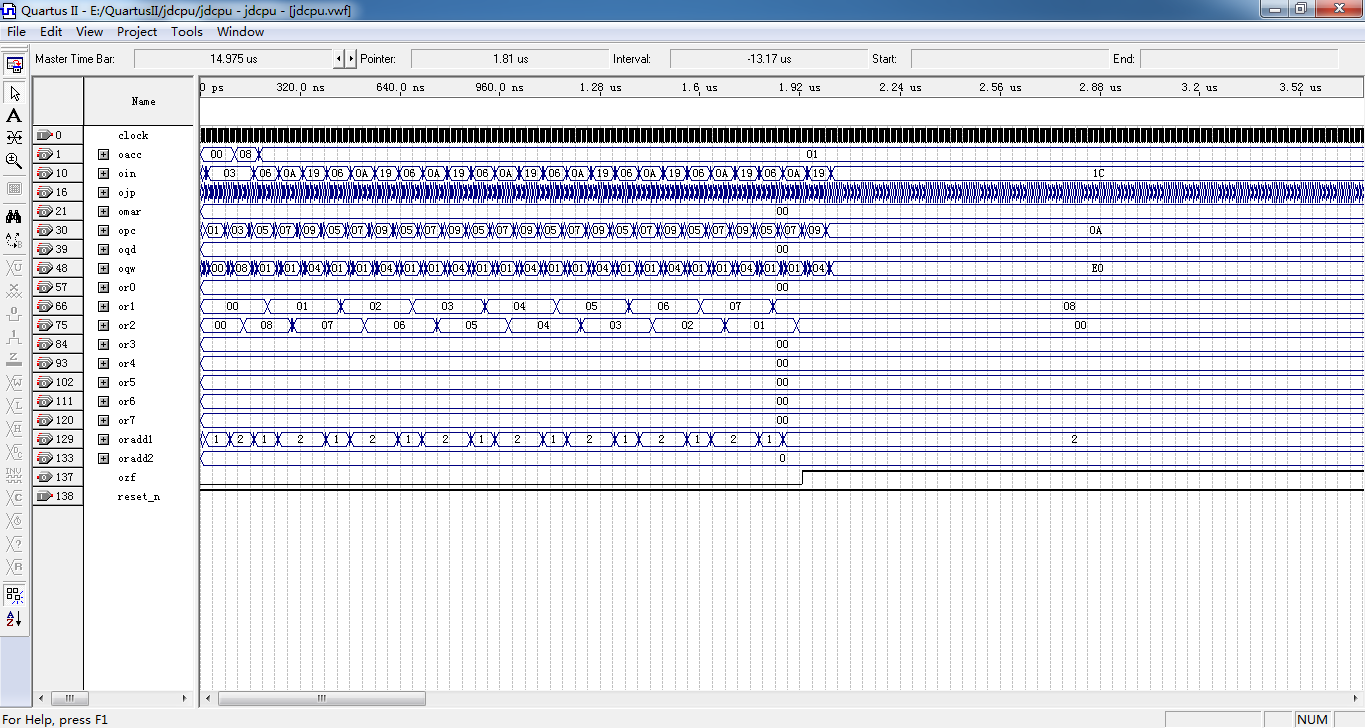
\includegraphics[scale=0.45]{vector.png}
\caption{仿真输出波形}
\end{figure}

\chapter{附录}
\section{操作时间表}

\clearpage


\newgeometry{a4paper,centering,top=0.8cm,bottom=1cm}

\begin{landscape}
\pagestyle{empty}
\begin{center}
\scalebox{0.80}[1]{
\begin{tabular}{|c|c|c|c|c|c|c|c|c|c|c|c|c|c|c|c|c|c|c|c|c|c|c|}
\hline
工作周期标记                   & 节拍                  & 状态条件 & 微操作命令信号                              & $\mathrm{mov_0}$ & $\mathrm{mov_1}$ & $\mathrm{mov_2}$ & $\mathrm{mov_3}$ & $\mathrm{add_0}$ & $\mathrm{add_1}$ & $\mathrm{add_2}$ & $\mathrm{sub_0}$ & $\mathrm{sub_1}$ & $\mathrm{sub_2}$ & $\mathrm{and_0}$ & $\mathrm{and_1}$ & $\mathrm{and_2}$ & $\mathrm{or_0}$ & $\mathrm{or_1}$ & $\mathrm{or_2}$ & not & jmp & hlt \\ \hline
\multirow{11}{*}{FE(取指)} & \multirow{5}{*}{T0} &      & M(PC)$\to$MDR              & 1    & 1    & 1    & 1    & 1    & 1    & 1    & 1    & 1    & 1    & 1    & 1    & 1    & 1   & 1   & 1   & 1   & 1   & 1   \\ \cline{3-23} 
                         &                     &      & MDR$\to$IR                 & 1    & 1    & 1    & 1    & 1    & 1    & 1    & 1    & 1    & 1    & 1    & 1    & 1    & 1   & 1   & 1   & 1   & 1   & 1   \\ \cline{3-23} 
                         &                     &      & OP(IR)$\to$IS          & 1    & 1    & 1    & 1    & 1    & 1    & 1    & 1    & 1    & 1    & 1    & 1    & 1    & 1   & 1   & 1   & 1   & 1   & 1   \\ \cline{3-23} 
                         &                     &      & Ad(IR)$\to$RADD1           & 1    & 1    & 1    & 1    & 1    & 1    & 1    & 1    & 1    & 1    & 1    & 1    & 1    & 1   & 1   & 1   &     &     &     \\ \cline{3-23} 
                         &                     &      & PC+1$\to$PC                & 1    & 1    & 1    & 1    & 1    & 1    & 1    & 1    & 1    & 1    & 1    & 1    & 1    & 1   & 1   & 1   &     & 1   &     \\ \cline{2-23} 
                         & T1                  &      & NOP                                  & 1    & 1    & 1    & 1    & 1    & 1    & 1    & 1    & 1    & 1    & 1    & 1    & 1    & 1   & 1   & 1   & 1   & 1   & 1   \\ \cline{2-23} 
                         & \multirow{5}{*}{T2} &      & M(PC)$\to$MDR              & 1    & 1    & 1    & 1    & 1    & 1    & 1    & 1    & 1    & 1    & 1    & 1    & 1    & 1   & 1   & 1   &     & 1   &     \\ \cline{3-23} 
                         &                     &      & MDR$\to$IR                 & 1    & 1    & 1    & 1    & 1    & 1    & 1    & 1    & 1    & 1    & 1    & 1    & 1    & 1   & 1   & 1   &     & 1   &     \\ \cline{3-23} 
                         &                     &      & OP(IR)$\to$ACC             &      &      &      & 1    &      &      & 1    &      &      & 1    &      &      & 1    &     &     & 1   &     & 1   &     \\ \cline{3-23} 
                         &                     &      & Ad(IR)$\to$RADD2           & 1    &      &      &      & 1    &      &      & 1    &      &      & 1    &      &      & 1   &     &     &     &     &     \\ \cline{3-23} 
                         &                     &      & Ad(IR)$\to$MAR             &      & 1    & 1    &      &      & 1    &      &      & 1    &      &      & 1    &      &     & 1   &     &     &     &     \\ \hline
\multirow{4}{*}{IND(间址)} & T0                  &      & NOP                                  & 1    & 1    & 1    & 1    & 1    & 1    & 1    & 1    & 1    & 1    & 1    & 1    & 1    & 1   & 1   & 1   & 1   & 1   & 1   \\ \cline{2-23} 
                         & \multirow{2}{*}{T1} &      & M(MAR)$\to$MDR             &      & 1    & 1    &      &      & 1    &      &      & 1    &      &      & 1    &      &     & 1   &     &     &     &     \\ \cline{3-23} 
                         &                     &      & OP(MDR)$\to$ACC            &      & 1    & 1    &      &      & 1    &      &      & 1    &      &      & 1    &      &     & 1   &     &     &     &     \\ \cline{2-23} 
                         & T2                  &      & NOP                                  & 1    & 1    & 1    & 1    & 1    & 1    & 1    & 1    & 1    & 1    & 1    & 1    & 1    & 1   & 1   & 1   & 1   & 1   & 1   \\ \hline
\multirow{9}{*}{EX(执行)}  & T0                  &      & M(RADD2)$\to$ACC           & 1    &      &      &      & 1    &      &      & 1    &      &      & 1    &      &      & 1   &     &     &     &     &     \\ \cline{2-23} 
                         & \multirow{6}{*}{T1} &      & ACC$\to$M(RDD1)            & 1    & 1    & 1    & 1    &      &      &      &      &      &      &      &      &      &     &     &     &     &     &     \\ \cline{3-23} 
                         &                     &      & M(RDD1)+ACC$\to$M(RADD1)   &      &      &      &      & 1    & 1    & 1    &      &      &      &      &      &      &     &     &     &     &     &     \\ \cline{3-23} 
                         &                     &      & M(RDD1)-ACC$\to$M(RADD1)   &      &      &      &      &      &      &      & 1    & 1    & 1    &      &      &      &     &     &     &     &     &     \\ \cline{3-23} 
                         &                     &      & M(RDD1)\&ACC$\to$M(RADD1)  &      &      &      &      &      &      &      &      &      &      & 1    & 1    & 1    &     &     &     &     &     &     \\ \cline{3-23} 
                         &                     &      & M(RDD1)|ACC$\to$M(RADD1)   &      &      &      &      &      &      &      &      &      &      &      &      &      & 1   & 1   & 1   &     &     &     \\ \cline{3-23} 
                         &                     &      & $\neg$M(RDD1)$\to$M(RADD1) &      &      &      &      &      &      &      &      &      &      &      &      &      &     &     &     & 1   &     &     \\ \cline{2-23} 
                         & \multirow{2}{*}{T2} &      & ACC$\to$PC                 &      &      &      &      &      &      &      &      &      &      &      &      &      &     &     &     &     & 1   &     \\ \cline{3-23} 
                         &                     &      & PC+1$\to$PC                & 1    & 1    & 1    & 1    & 1    & 1    & 1    & 1    & 1    & 1    & 1    & 1    & 1    & 1   & 1   & 1   & 1   & 1   &     \\ \hline
\end{tabular}
}
\end{center}
\end{landscape}

\end{document}